\documentclass[12pt,a4paper]{article}
\title{MATH1110 Lec 009 Week 6-F}
\author{Benjamin Thompson}
\date{October 1, 2021}

\usepackage[left=2cm,right=2cm]{geometry}

\usepackage{tikz, tikz-3dplot}
\usetikzlibrary{arrows.meta,decorations.markings}
\usepackage{etoolbox}

\usepackage{pgfplots}

\pgfplotsset{every axis/.append style={
axis x line=middle,    % put the x axis in the middle
axis y line=middle,    % put the y axis in the middle
axis line style={-{Stealth[length=3mm]},color=black}, % arrows on the axis
minor tick num=1
}}

\usepackage{amsmath}
\usepackage{graphicx}

\usepackage{fancyhdr}
\pagestyle{fancy}

\newcommand{\rar}{\rightarrow}

\fancyhf{}
\lhead{MATH1110 Sec 009}
\chead{Week 6-F}
\rhead{October 1, 2021}
\cfoot{}

\begin{document}
\section*{Quiz and Solutions}
\subsection*{Problems}
\begin{enumerate}
    \item Evaluate
    \[
        \lim_{\theta \rightarrow 0} \frac{\theta}{\tan \theta}
    \]
    if it exists. If it does not, explain why.
    \item The tangent to the curve $y = x^2$ at $x = 10$ intersects the $x$-axis. Find this intersection point.
    \item Let \[
    f(x) = \begin{cases}
        x + 1 & x < 0 \\
        1 - x^2 & x \geq 0. 
    \end{cases}
    \] Is $f$ differentiable at $x = 0$? Why / why not?
    \item Does $(pq)' = p'q'$ for all polynomials $p(x),q(x)?$ If not, give a pair of polynomials $(a(x),b(x))$ for which $(ab)' \ne a'b'$.
    \item A polynomial $p(x)$, as well as its derivative $p'(x)$ and second derivative $p''(x)$ are plotted below. Match $p,p',p''$ with $A,B,C$.
\[
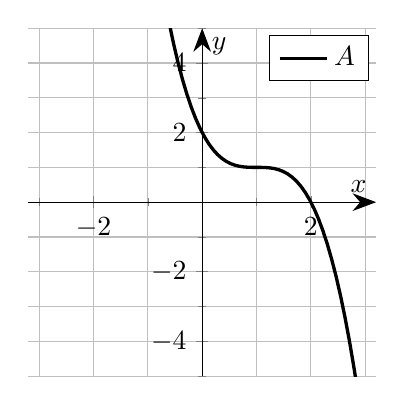
\begin{tikzpicture}
\begin{axis}[xlabel={$x$},ylabel={$y$},width=6cm, height=6cm, xmin=-3.2,xmax=3.2, ymin=-5,ymax=5, grid=both]
\addplot [very thick, domain=-4:4,samples=100]{-1*(x-1)^3 + 1};
\addlegendentry{$A$}
\end{axis}
\end{tikzpicture}
\quad
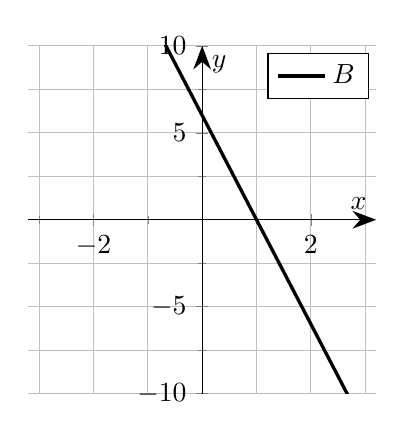
\begin{tikzpicture}
\begin{axis}[xlabel={$x$},ylabel={$y$},width=6cm, height=6cm, xmin=-3.2,xmax=3.2, ymin=-10,ymax=10, grid=both]
\addplot [very thick, domain=-4:4,samples=100]{-6*(x-1)};
\addlegendentry{$B$}
\end{axis}
\end{tikzpicture}
\quad
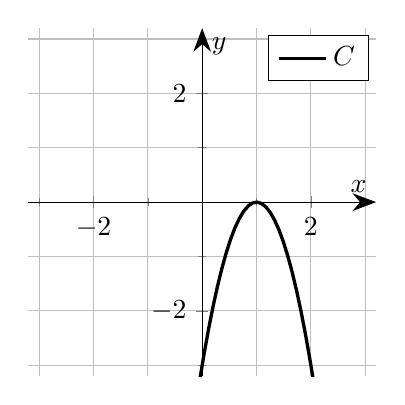
\begin{tikzpicture}
\begin{axis}[xlabel={$x$},ylabel={$y$},width=6cm, height=6cm, xmin=-3.2,xmax=3.2, ymin=-3.2,ymax=3.2, grid=both]
\addplot [very thick, domain=-4:4,samples=100]{-3*(x-1)^2};
\addlegendentry{$C$}
\end{axis}
\end{tikzpicture}
\]
\end{enumerate}
\subsection*{Solutions}
\begin{enumerate}
	\item Using the identity $\tan \theta = \sin \theta / \cos \theta$, we can do some rearranging:
\[
	\frac{\theta}{\tan \theta} = \frac{\theta}{\frac{\sin \theta}{\cos \theta}} = \frac{\theta \cos \theta}{\sin \theta} = \cos \theta \cdot \frac{1}{\frac{\sin \theta}{\theta}}.
\]
Since $\lim_{\theta \rar 0} \sin \theta / \theta = 1 \ne 0$, 
\[
	\lim_{\theta \rar 0} \frac{1}{\frac{\sin \theta}{\theta}} = \frac{1}{1} = 1.
\]
The function $\cos \theta$ is continuous, so $\lim_{\theta \rar 0} \cos \theta = \cos(0) = 1$. We can then apply the product limit law to conclude
\[
	\lim_{\theta \rar 0} \left( \cos \theta \cdot \frac{1}{\frac{\sin \theta}{\theta}} \right) = \left( \lim_{\theta \rar 0} \cos \theta \right) \left( \lim_{\theta \rar 0} \frac{1}{\frac{\sin \theta}{\theta}} \right) = 1 \cdot 1 = 1.
\]
	\item Since $f'(x) = 2x$, $f'(10) = 20$, so the gradient of the tangent line to the curve $y = x^2$ at $x = 10$ is 20.

 A non-vertical line with gradient $m$ passing through a point $(x_0,y_0)$ has equation $y - y_0 = m(x - x_0)$.

The tangent line touches the curve at $(10,100)$ and therefore passes through this point. Therefore the equation of the tangent line is $y - 100 = 20(x - 10)$. Expanding the RHS of this equation and rearranging this gives $y = 20x - 100$.

Every point on the $x$-axis has a $y$-value of 0, so to find the intersection point of the tangent line with the $x$-axis we substitute $y = 0$ into the equation of the line and solve for $x$:
\begin{equation*}
\begin{split}
		&0 	= 20x - 100 \\
		&\Rightarrow 20x = 100 \\
		&\Rightarrow x = 100/20 = 5.
\end{split}
\end{equation*}
	\item Since $(x + 1)' = 1$ while $(1 - x^2)' = -2x$, and $1 \ne -2x$ at $x = 0$, we can expect that the derivative will not exist at $x = 0$. We can formally prove this using the limit definition of the derivative and computing left and right-handed limits:
\[
	\lim_{h \rar 0^-} \frac{f(0 + h) - f(0)}{h} = \lim_{h \rar 0^-} \frac{(1 + h) - 1}{h} = \lim_{h \rar 0}{1} = 1,
\]
\[
	\lim_{h \rar 0^+} \frac{f(0 + h) - f(0)}{h} = \lim_{h \rar 0^+} \frac{1 - (0 + h)^2 - 1}{h} = \lim_{h \rar 0^+} \frac{-h^2}{h} = -\lim_{h \rar 0^+} h = 0.
\]
Since the left-hand and right-hand limits are not equal, the overall limit does not exist, so $f$ is not differentiable at $x = 0$.
	\item Certainly not. Let $a(x) = b(x) = x$. Then
\[
	(ab)' = (x^2)' = 2x \ne 1 = 1\cdot 1 = a'b'.
\]
	\item Since $B$ is a plot of a line, $B'$ is constant. Neither $A$ nor $C$ is a constant function, so $B' \ne A$ and $B' \ne C$, which means $B = p''$.

Note that $C$ has a horizontal tangent line at $x = 1$, so $C'$ must be 0 at $x = 1$. Looking at the plots, we see $B$ is 0 at $x = 1$ but $A$ is non-zero at $x = 1$, so $C' = B$. Hence $C = p'$. It follows that $(A,B,C) = (p,p'',p)$.
\end{enumerate}

\end{document}
